\section{Background}
\label{sec:background}

\subsection{Single-Input Multiple-Output}
\label{sec:simo}

Wireless devices have transitioned to using multiple antennas to leverage gains from on both client devices and access points.
These are known as multiple-input multiple-output (MIMO) systems and their design involves using simultaneous transmissions and receptions from different antennas to obtain higher throughput, than what would be possible using any given pair of antennas on a transmitter and receiver.
MIMO systems can provide higher throughput and resilience due to their ability to coherently combine signals both at the transmitter (known as \textit{beamforming}) and the receiver (known as \textit{diversity}).
In traditional MIMO system such as those found in 802.11n, the various receiver antennas are a part of the same device which makes it easier to synchronize and combine the different receiver channels.
However, distributed MIMO systems allow the receivers to be completely independent devices and still be able to coherently combine the received signals.
Single-input multiple-output (SIMO) as shown in \figref{simo} is a subset of distributed MIMO systems where the transmitter only uses a single antenna.
The LoRaWAN scenario we explore in this paper is based on SIMO systems.

\begin{figure}[!htb]
    \centering
    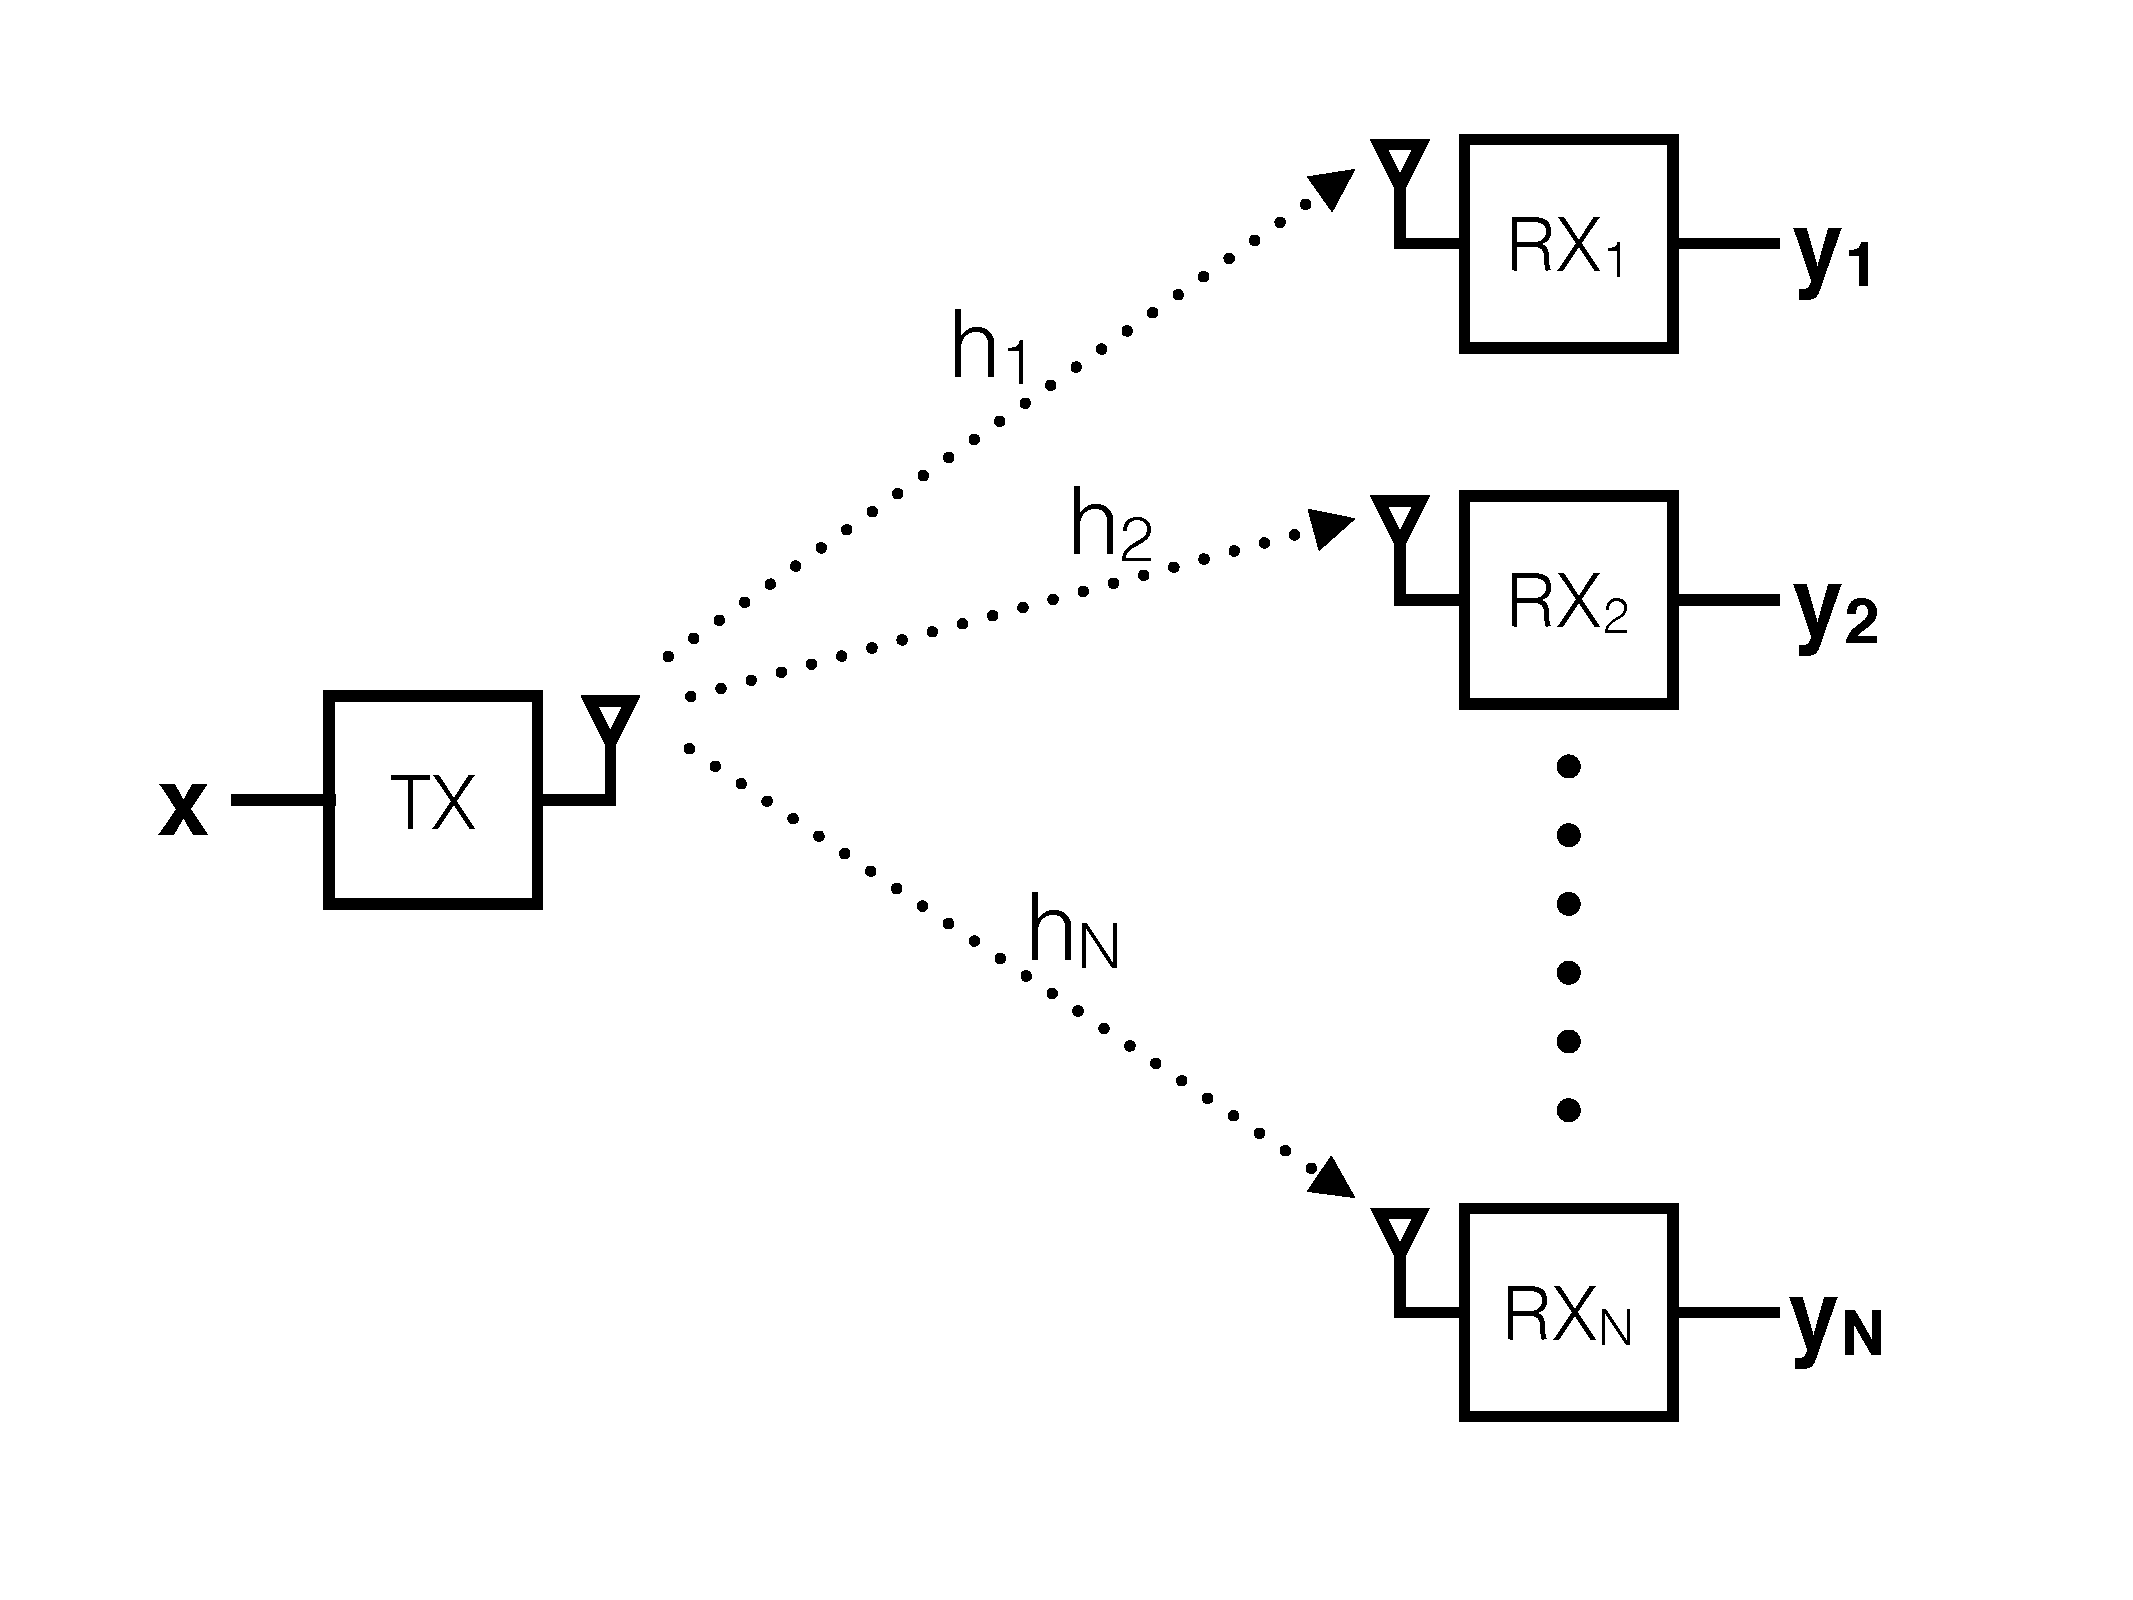
\includegraphics[width=0.45\textwidth]{figures/SIMO}
    \caption{A single-input multiple-output (SIMO) wireless system}
    \label{fig:simo}
\end{figure}

Let the transmitted signal be $x$ and each of the gateways receive a signal $y_i$ through an AWGN channel that introduces independent noise $n_i$ at the receivers.
Since LoRa modulated signals are narrowband (up to 500 $kHz$) and their symbol periods are large ({\color{blue} Add number}) to remain unaffected by inter-symbol interference, we get the following simplified channel model.

\begin{align*}
y_i &= h_i x_i + n_i \\
\therefore h^*_i y_i &= h^*_i h_i x_i + h^*_i n_i \\
	&= \left| h_i \right|^2 x + n'_i
\end{align*}

Estimating the $h_i$ is only based on information available locally to the receiver.
The combined signals can then be coalesced by a joint decoder

\begin{align*}
y_{\text{combined}} = 
	&= \sum_{i=1}^N h^*_i y_i \\
	&= \sum_{i=1}^N \left| h_i \right|^2 x + \sum_{i=1}^N h^*_i n_i
\end{align*}

The first term is the combined signal while the second term is the combined
noise. However, the signals add up coherently while the noise, being
independent, adds up incoherently. This results in an overall increase in the
combined SNR which allows us to jointly decode a packet that would otherwise
not be decodable by any individula receiver.

\begin{align*}
SNR_{\text{combined}} &= \frac{\text{total signal power}}{\text{total noise power}} \\
	&= \frac{\left| \sum_{i=1}^N \left| h_i \right|^2 x \right|^2}{\sum_{i=1}^N \left| h^*_i n_i \right|^2} \\
	&\geq \frac{\left| \left| h_i \right|^2 x \right|^2}{\left| h^*_i n_i \right|^2} = SNR_i
\end{align*}

\subsection{LoRa}
\label{sec:lora}

LoRa is a chirp spread-spectrum modulation scheme developed by Semtech for low bit rate, long range communication.

{\color{blue}
Packet structure

Encoding as chirps

Spreading factors

How this enables power savings
}

A unique aspects of LoRa systems is that the gateway chipsets can demodulate on multiple channels and at multiple data rates simultaneously.

\subsection{LoRaWAN}
\label{sec:lorawan}

The LoRa Wide-Area Networking (LoRaWAN) protocol works on top of the LoRa
modulation layer to create an LP-WAN network capable of bi-directional data
transfer. Its functionality is analogous to the Networking and transport
layers (layers three and four) in the typical OSI design. LoRaWAN networks
are designed to be simple star-topologies that have client devices directly
communicating with a gateway that is connected to the internet over ethernet
or cellular links. LoRaWAN defines three main device classes: bi-directional
end-devices with downlink followed by uplink (Class A), bi-directional
end-devices with transmission slots scheduled for downlink (Class B) and
always-on bi-directional devices (Class C). Class A is primarily intended for
sensors, Class B is intended for sensors with actuators while Class C is
intended for powered devices that require low-latency. Gateways are very
simple and relatively inexpensive forwarders that send received packets to a
cloud LoRaWAN server and can be commanded by the server to transmit data to
clients at a specific time. Packet decoding, managing acknowledgements and
MAC parameters like data-rate and power-level are decided at a LoRaWAN
server. The LoRa community often refers to the system as having a
``MAC-in-the-Cloud" design.

LoRaWAN allows and encourages its users to deploy their own gateways. In this
paper, we refer to these as user-deployed gateways (UGW). These UGWs are
completely unplanned and on low-bandwidth, unreliable internet connections
(compared to cellular base-stations which are extensively planned and have
dedicated optic fiber connections). In pilot deployments, we've observed the
same transmission being received by multiple gateways. In this paper, we
leverage this observation combined with the diversity from unplanned UGW
deployments to extend the coverage of higher data-rates in our network.
Low-power devices which can now transmit at higher data rates thus end up
saving energy to shorter transmit time.

{\color{blue}

Q. how do we save client power while sticking to LoRaWAN?
}